\documentclass[10pt]{article}

% Pacotes extras necessários
\usepackage{amsmath}
\usepackage[lmargin=0.5in, rmargin=0.5in, tmargin=0.5in, bmargin=0.5in, includehead, includefoot]{geometry}
\usepackage{amsfonts}
\usepackage[utf8]{inputenc}
\usepackage[portuguese]{babel}
\usepackage{graphicx}
\usepackage{fancyhdr}
\usepackage{setspace}
\usepackage{listings}
\usepackage{url}
\usepackage{enumitem}
\usepackage{appendix} % For creating appendix sections

% More defined colors
\usepackage[dvipsnames]{xcolor}

% Define a custom style for the code listing
\lstdefinestyle{mystyle}{
    language=Octave,
    backgroundcolor=\color{white},   % Choose the background color
    basicstyle=\ttfamily\footnotesize, % Set the font and size for the code
    numbers=left,                    % Line numbers on the left
    numberstyle=\tiny\color{gray},   % Line numbers style
    numbersep=5pt,                   % Distance of line numbers from the code
    tabsize=2,                       % Set tab size (default is 8 spaces)
    breaklines=true,                 % Automatically wrap long lines
    keywordstyle=\color{blue},       % Keywords in blue
    commentstyle=\color{green!60!black}, % Comments in green
    stringstyle=\color{orange},      % Strings in orange
    frame=single,                    % Draw a frame around the code
    keepspaces=true,                 % Preserve spaces in text
    showspaces=false,                % Don't show spaces in strings
    showstringspaces=false,          % Don't show spaces in strings
    showtabs=false,                  % Don't show tabs in strings
    % Add any other options you need
}

\lstset{style=mystyle} % Set the custom style
 
% Required package
\usepackage{tikz}
\usetikzlibrary{positioning}

\graphicspath{ {./images/} }

% Sets para outras partes
\setlength{\parindent}{0pt}
\setstretch{1.5}
\DeclareMathOperator{\sen}{sen}
\DeclareMathOperator{\sinc}{sinc}

%% Facilidades
%% -- Laplace
\newcommand{\Lap}[1]{\mathcal{L}\left\{#1\right\}}

%% -- Negrito em matemáticas
\newcommand{\bm}[1]{\boldsymbol{#1}}


% ------- Estilo do trabalho -------- %
\fancypagestyle{capa}{
    \fancyhf{}
    \renewcommand\headrulewidth{0pt}
}

\pagestyle{fancy}
\fancyhead{}
\fancyhead[L]{\thepage}
\fancyfoot{}
% ----------------------------------- %

% Dados do Grupo
\title{Modelagem de Sistemas Dinâmicos - Trabalho Nº4}
\author{
    Leonardo Soares da Costa Tanaka - DRE: 121067652 \\
    Engenharia de Controle e Automação/UFRJ \\
    Rio de Janeiro, Brasil \\
    Julho de 2023
}
\date{}

\begin{document}
\maketitle
\thispagestyle{capa}

\quad Para este trabalho, vamos utilizar o arquivo “trabalho4-2023-1.mat” que tem os sinais de entrada u(t) e de saída y(t) de um sistema
linear contínuo com função de transferência G(s). Os sinais u e y foram aplicados e aquisitados
com uma frequência de amostragem fs = 2Hz (período de amostragem T = 0.5s). A variável
independente tempo t é o vetor com os instantes que foram realizadas as amostragens dos
sinais u(t) e y(t).

\quad Vale notar que o sinal de saída y(t) está quantizado e contaminado com ruído.

\section{FFT}

\quad Determinando, utilizando a FFT (Fast Fourier Transform), o espectro do sinal de entrada
(módulo e fase) em função da frequência em Hz. Utilizando o Matlab para coletar os dados,
utilizar a FFT, calcular os espectros do sinal de entrada e plotar o gráfico.

\begin{figure}[h]
    \centering
    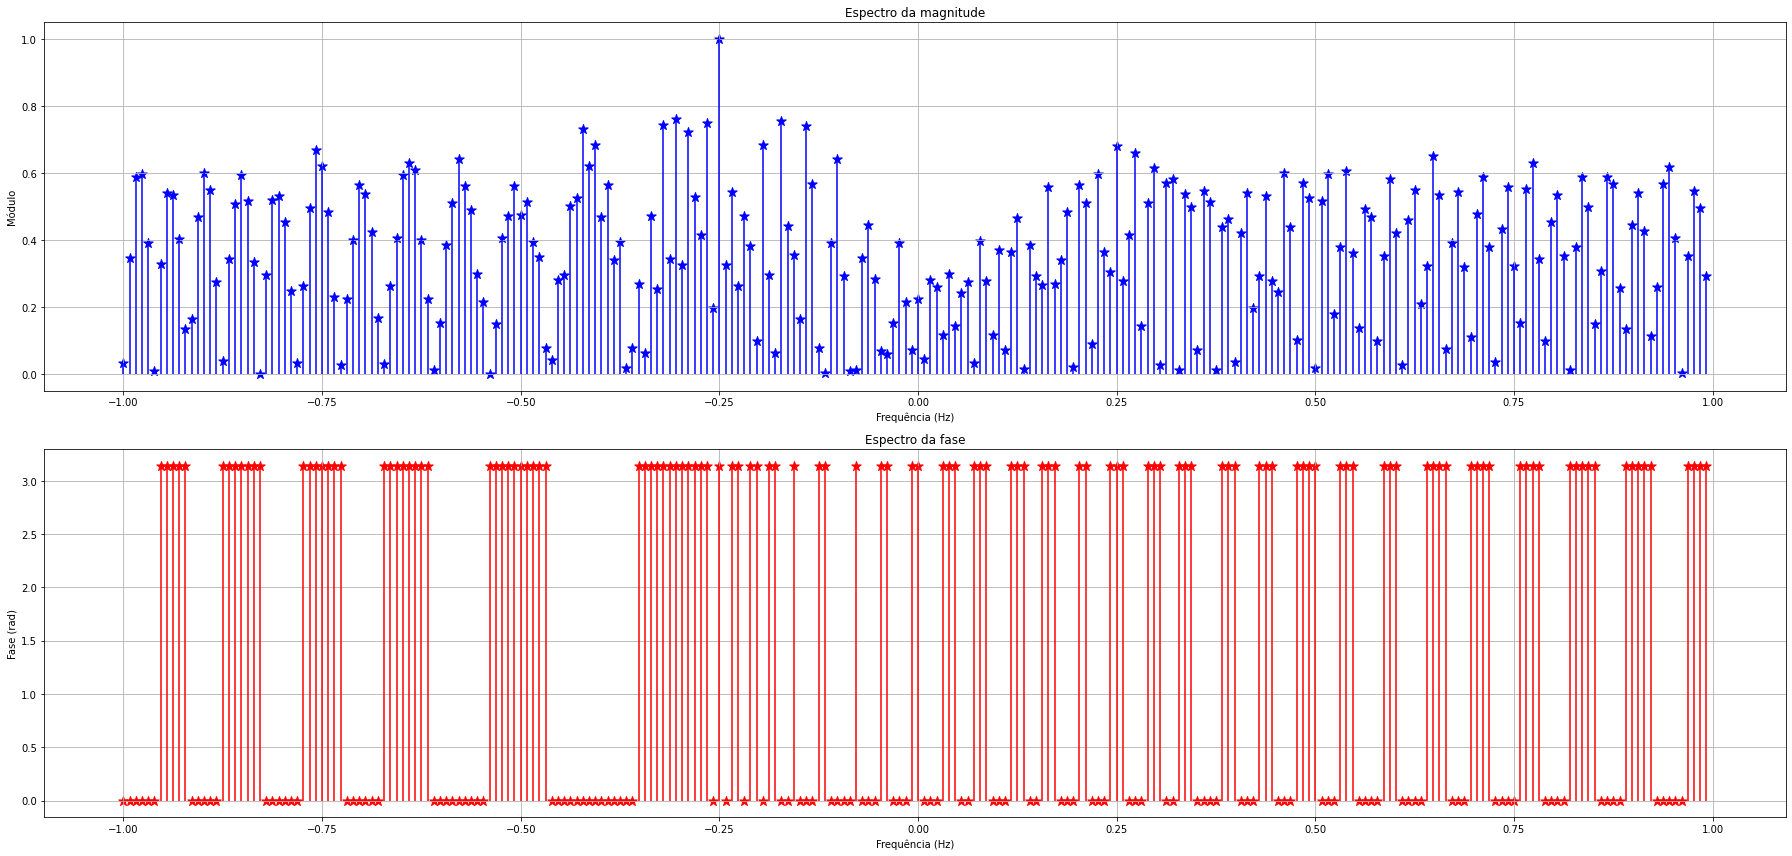
\includegraphics[scale=0.34]{fft.png}
    \caption{Espectros dos sinais da entrada}
\end{figure}

\quad É possível observar uma simetria no gráfico da mangnitude em torno de 1
com uma parte central com valores iguais a 2.61115 entre 0.4 e 1.6,
duas partes seguintes com valores iguais a 10.4446 entre (0.03 e 0.4) e (1.6 e 1.96) e duas
partes extremas com os mesmos valores que a parte central. Já no gráfico de fase, é possível
observar uma oscilação bem similar entre 0.4 e 1.6 e
outras oscilações similares entre (0.03 e 0.4) e (1.6 e 1.96) com valores entre $-\pi$ e $\pi$.

\section{Resposta em frequência do sistema G(jw)}

\quad Estimando a resposta em frequência do sistema G(jw) utilizando os espectros dos sinais
de entrada U(jw) e de saída Y(jw):

\begin{figure}[h]
    \centering
    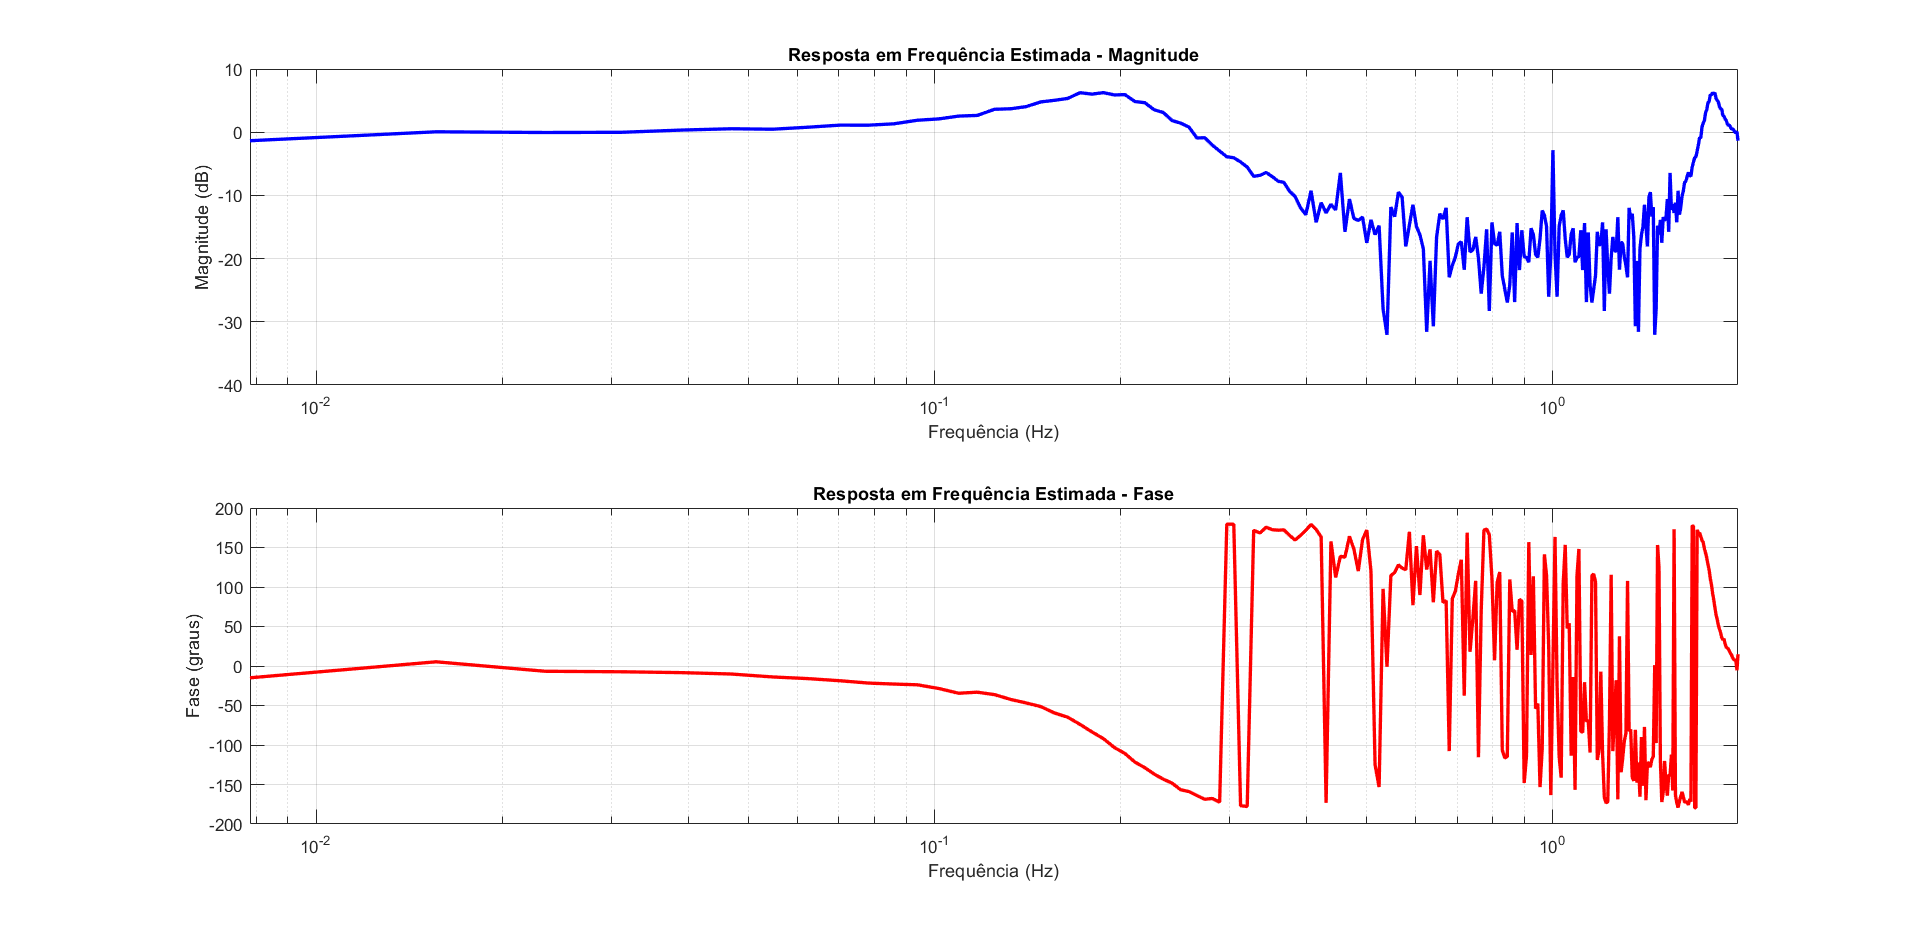
\includegraphics[scale=0.34]{g.png}
    \caption{Resposta em frequência do sistema G(jw)}
\end{figure}

\section{Principais caracteríticas da resposta em frequência}

\quad Ao visualizar gráfico de resposta em frequência é possível observar um sistema de segunda ordem entre 0.1 Hz e 0.3 rad/s,
Os sistemas de segunda ordem apresentam um comportamento ressonante em torno da frequência natural do sistema,
que é determinada pela constante de tempo e a frequência de amortecimento.
Se a frequência de excitação estiver próxima à frequência natural do sistema,
a resposta pode se tornar muito amplificada, criando um pico na resposta em frequência.

\quad Quanto ao ruído começando um pouco antes de 0.3 Hz e estendendo-se até mais de 2 Hz,
isso pode ter efeitos significativos na resposta do sistema,
especialmente se a amplitude do ruído for alta em comparação com o sinal de interesse.
O ruído pode mascarar a resposta do sistema,
dificultando a identificação precisa dos picos de ressonância ou
outros comportamentos relevantes.

\newpage

\section{Determinação do sistema de $2\textsuperscript{a}$ ordem}

\quad Para determinar o sistema de $2\textsuperscript{a}$ ordem que tem resposta em frequência mais próxima com a estimada,
foi feito diversos testes trocando as constantes $\zeta$ e $w_n$ até chegar numa visualização bem próxima entre as duas respostas em frequência.

\begin{figure}[h]
    \centering
    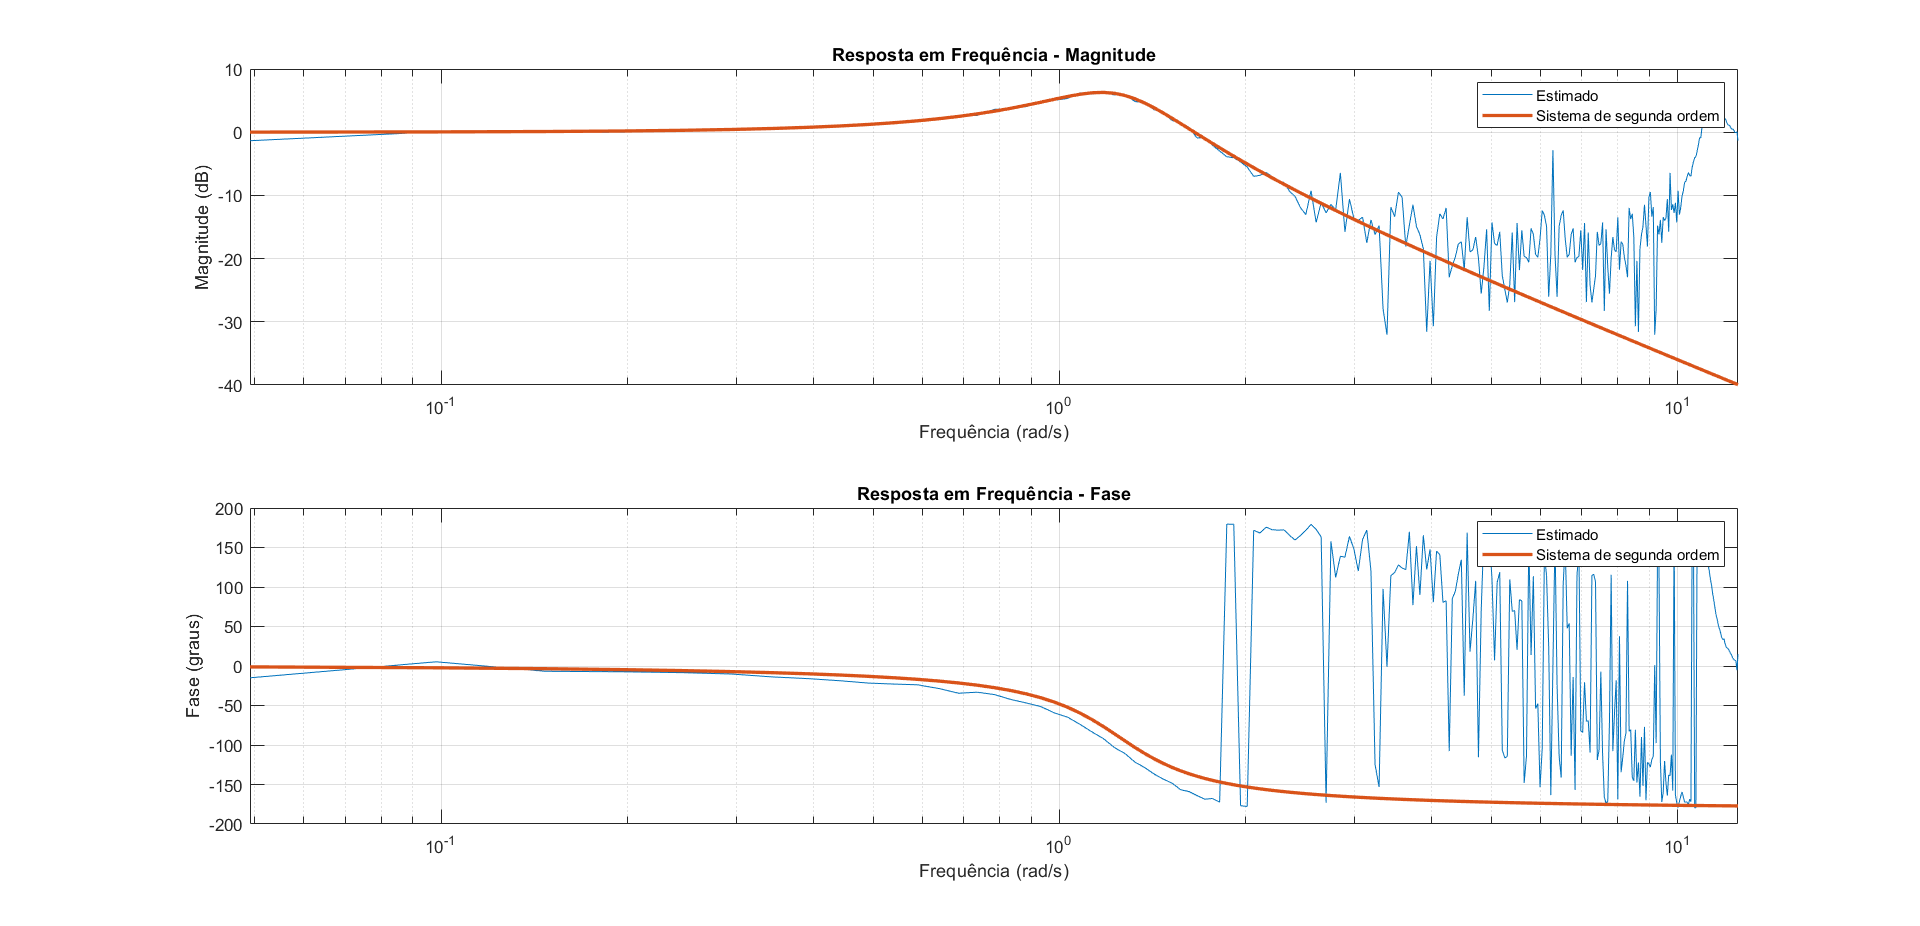
\includegraphics[scale=0.35]{g_manual.png}
    \caption{Resposta em frequência}
\end{figure}

\quad Foi utilizada a seguinte fórmula que representa a função de transferência de um sistema de $2\textsuperscript{a}$ ordem:

\begin{equation}
    G(s) = \frac{\omega_n^2}{s^2 + 2 \zeta \cdot \omega_n \cdot s + \omega_n^2}
\end{equation}

\quad Os valores obtidos foram:

\begin{equation}
    w_n = 1.25 \ e \ \zeta = 0.25
\end{equation}

\newpage

\section{System Identification Apps}

\quad Foi colocado os dados da entrada u(t) e saída y(t) que foram acessados pelo "System Identification Apps".

\begin{figure}[h]
    \centering
    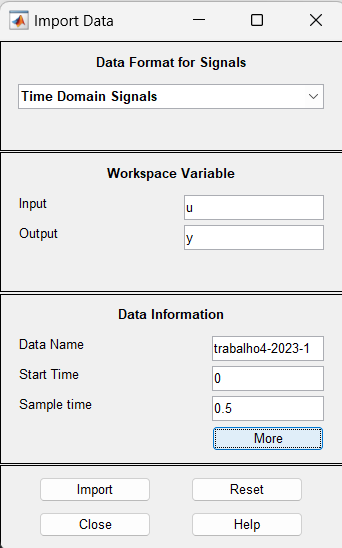
\includegraphics[scale=0.5]{si1.png}
\end{figure}

\quad Depois, disso foi colocado para estimar a função de transferência com nenhum zero e dois pólos.

\begin{figure}[h]
    \centering
    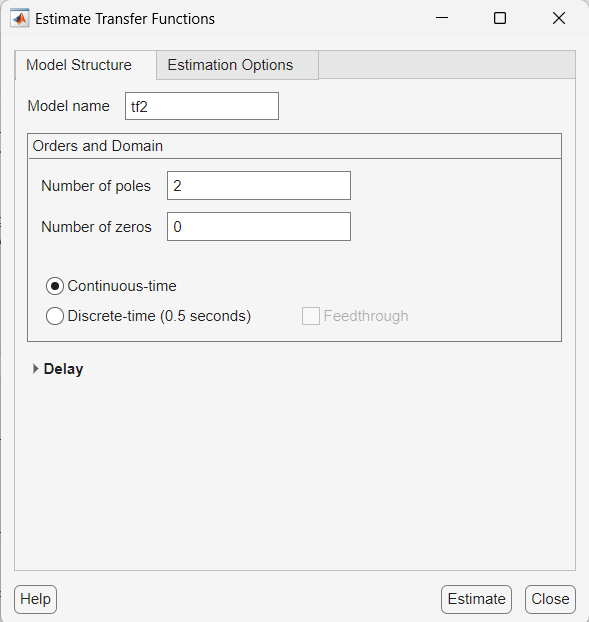
\includegraphics[scale=0.4]{si2.png}
\end{figure}

\quad Foi obtido o resultado pelo "System Identification Apps".

\begin{figure}[h]
    \centering
    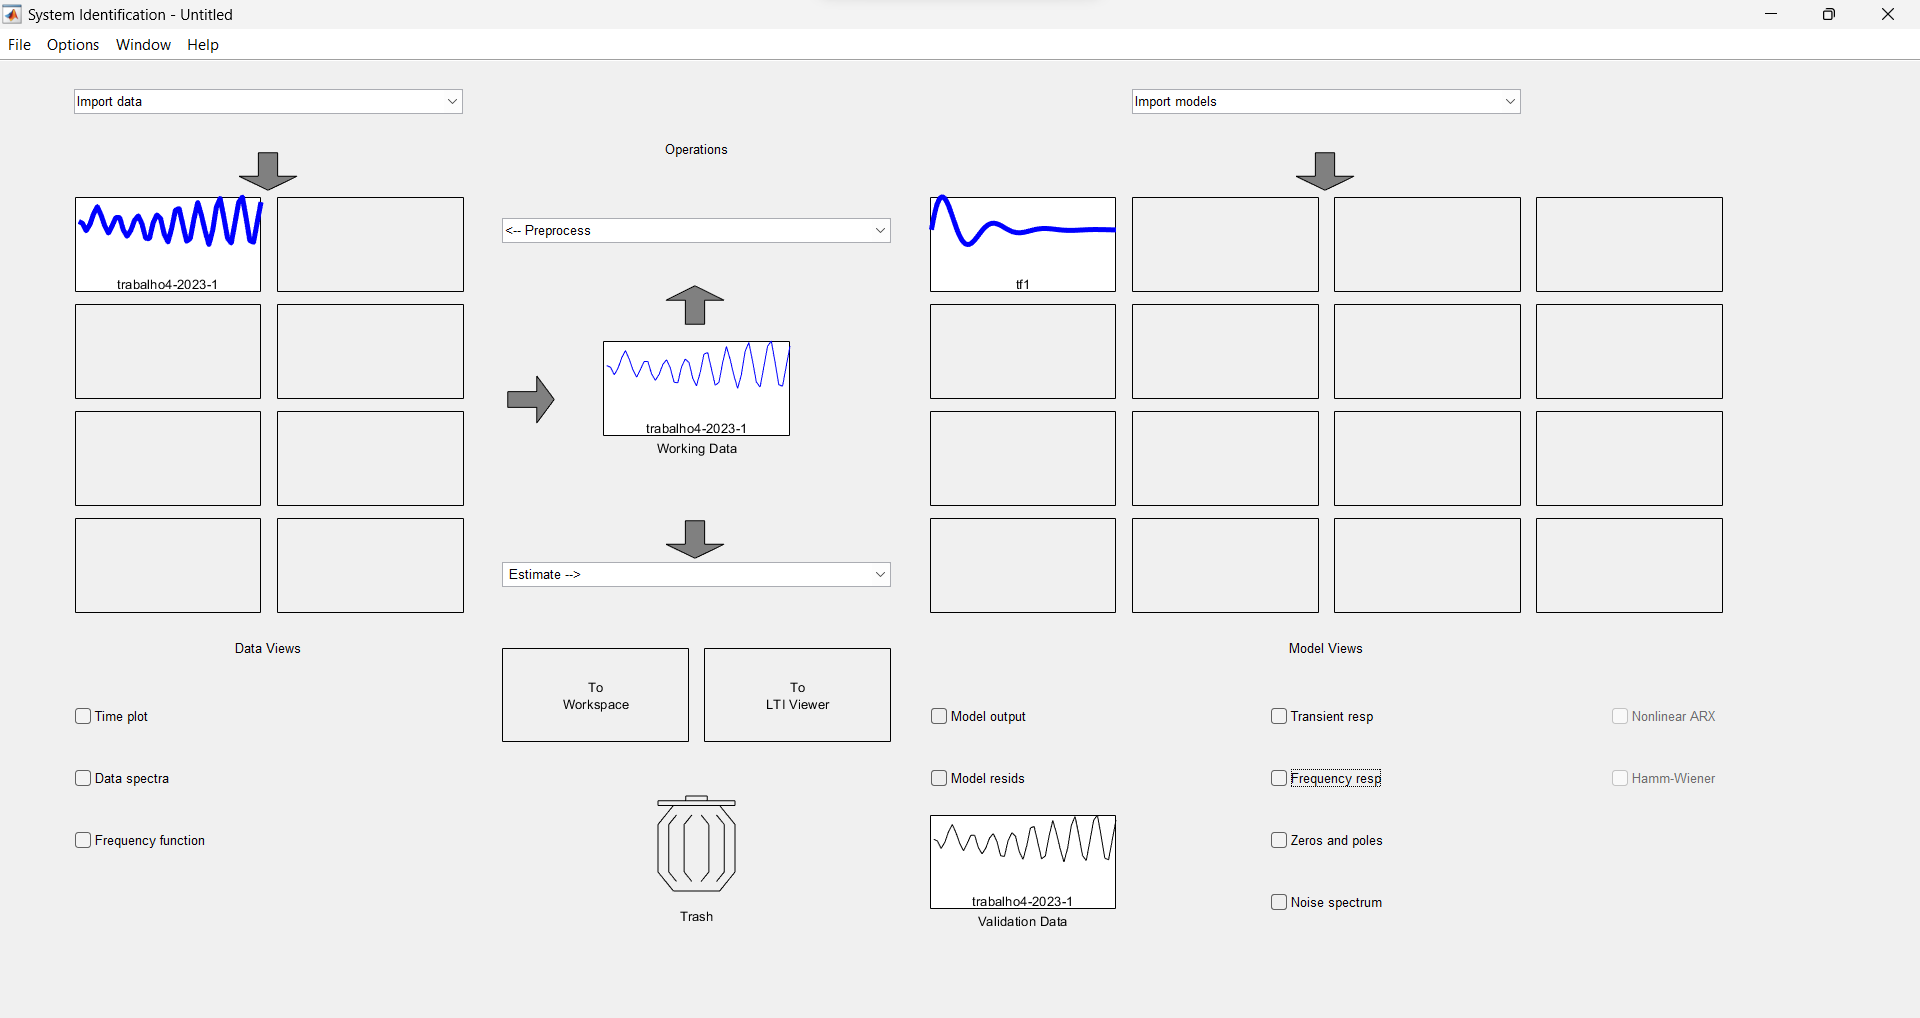
\includegraphics[scale=0.24]{si5.png}
    
\end{figure}

\newpage

\quad Resultados obtidos:

\begin{figure}[h]
    \centering
    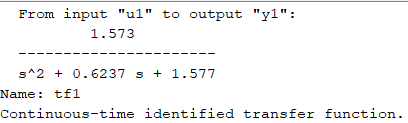
\includegraphics[scale=0.7]{si6.png}
    \caption{Função de transferência}
\end{figure}

\begin{figure}[h]
    \centering
    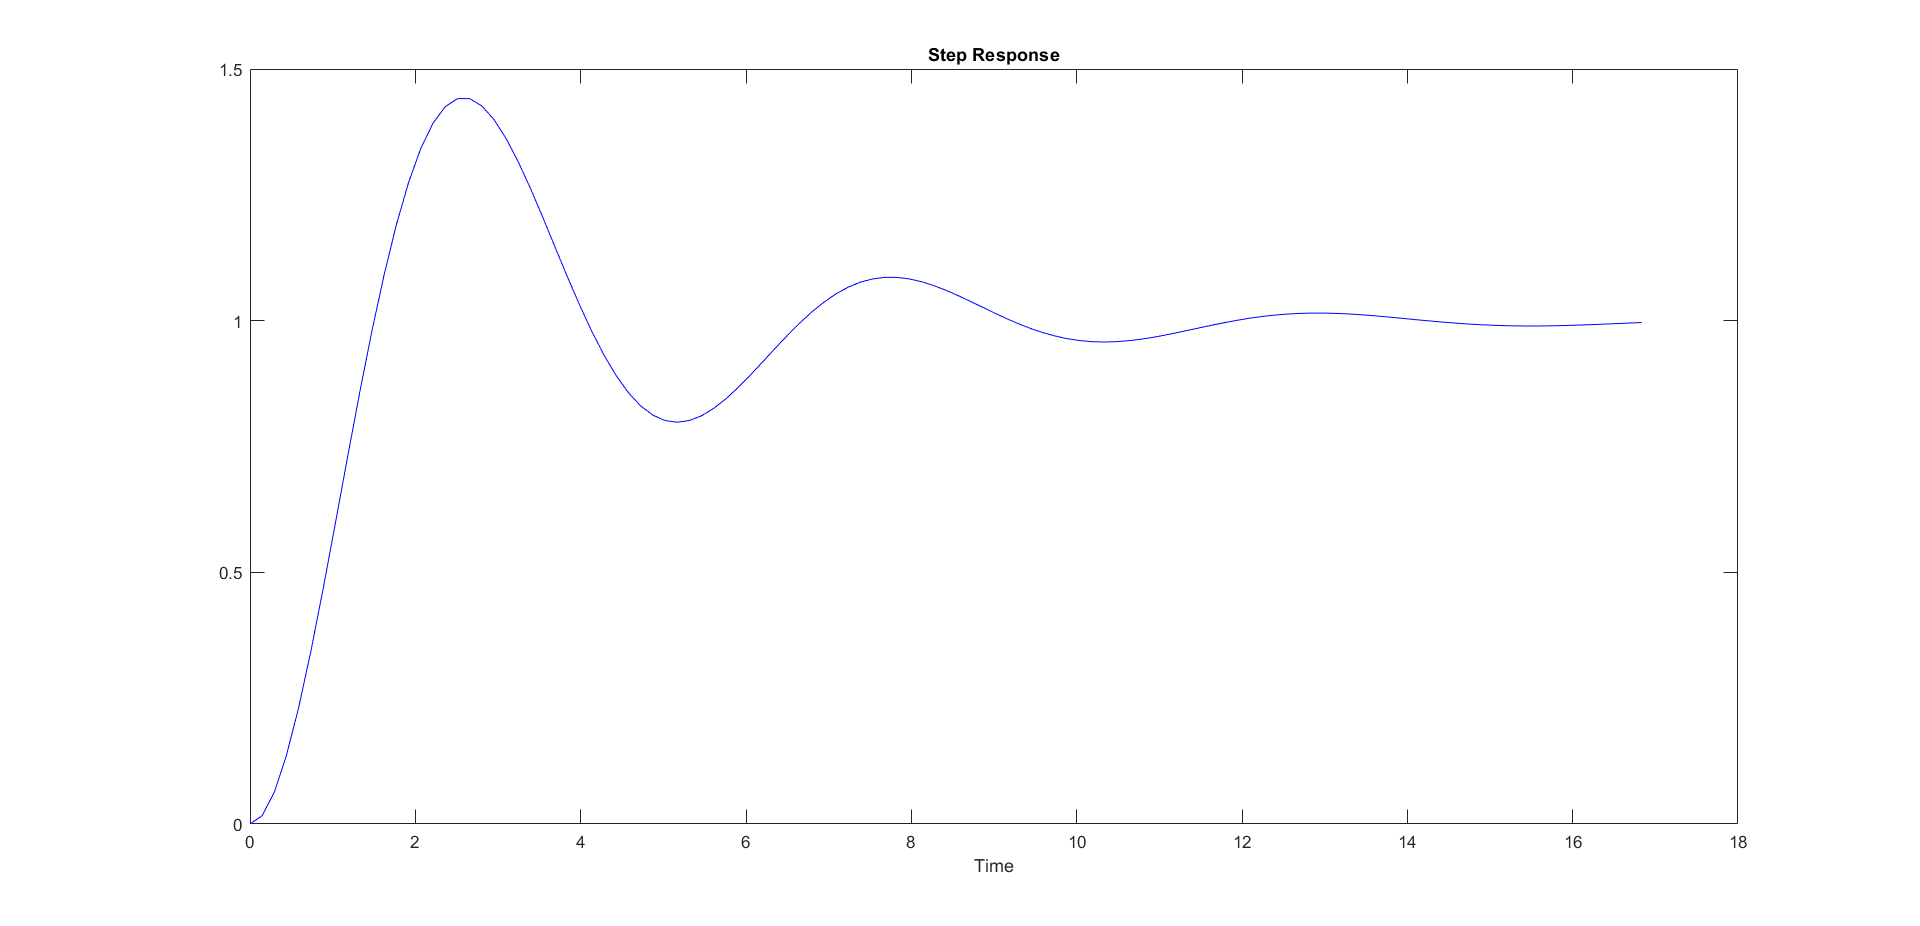
\includegraphics[scale=0.24]{si3.png}
    \caption{Resposta transiente}
\end{figure}

\begin{figure}[h]
    \centering
    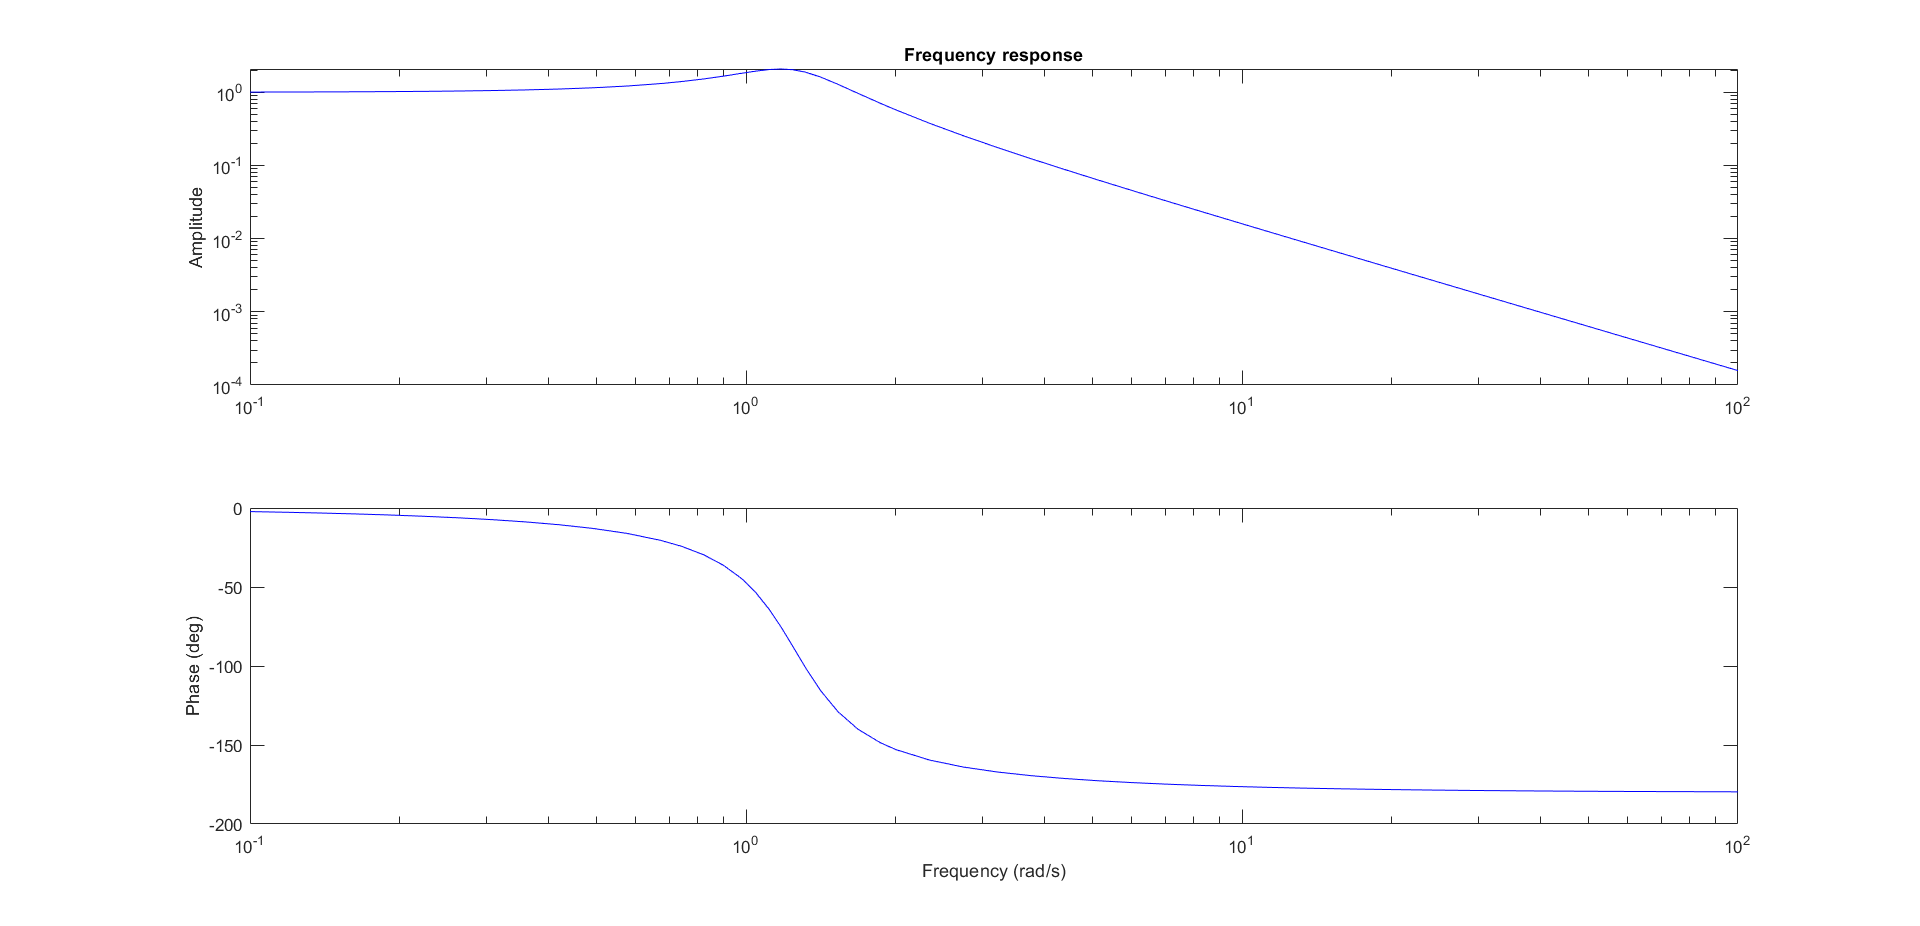
\includegraphics[scale=0.24]{si4.png}
    \caption{Resposta em frequência}
\end{figure}

\quad Como pode ser visto o resultado obtido pelo "System Identification Apps" ficou bem próximo ao resultado obtido no item anterior,
sendo bem similares na resposta em frequência.

\newpage

\section{Conclusão}

\quad Ao longo deste projeto, realizamos uma análise detalhada do sistema linear contínuo com função de transferência G(s),
utilizando sinais de entrada e saída adquiridos com uma frequência de amostragem fs = 2Hz.
Nossa análise incluiu a determinação do espectro do sinal de entrada por meio da Transformada Rápida de Fourier (FFT),
bem como a estimativa da resposta em frequência do sistema utilizando os espectros dos sinais de entrada U(jw) e de saída Y(jw).

\quad Os resultados da análise mostraram que o sinal de entrada apresenta certas características principais em seu espectro,
como picos de frequência em determinadas regiões e uma fase específica associada a cada componente frequencial.
Essas características podem ser cruciais para a compreensão do comportamento do sistema em diferentes faixas de frequência.

\quad Com base nas estimativas da resposta em frequência do sistema G(jw),
foi possível traçar o módulo e a fase da resposta em função da frequência em rad/s.
Essas curvas nos permitiram identificar as principais características da resposta em frequência,
incluindo picos de ressonância, frequência natural e frequência de amortecimento.

\quad Além disso, foi comparada a resposta em frequência estimada com os resultados obtidos por meio do "System Identification Apps" do Matlab.
Essa comparação permitiu validar os resultados e verificar a precisão das estimativas.

\quad No geral, este trabalho forneceu uma visão aprofundada sobre o comportamento do sistema estudado em termos de sua resposta em frequência.
Com as informações coletadas, pudemos identificar um modelo de segunda ordem que melhor se ajusta à resposta em frequência estimada.
Isso pode ser fundamental para futuras aplicações práticas do sistema ou para projetos de controle.

\quad No entanto, durante o projeto, foram encontrados alguns desafios, como ruído presente nos sinais adquiridos, que podem ter afetado a precisão das estimativas. Para mitigar esses problemas, foram empregadas técnicas específicas de análise de sinais e filtragem.
No entanto, é importante ressaltar que a qualidade dos resultados pode ser influenciada por essas limitações.

\quad Em conclusão, o trabalho proporcionou uma sólida compreensão do sistema estudado em termos de sua resposta em frequência,
identificando suas principais características e estimando um modelo de segunda ordem aproximado.
Espero que os resultados aqui apresentados possam ser úteis para futuros estudos e aplicações práticas no campo da engenharia de controle e automação.

\newpage

\begin{appendices}

\section{Código 1}

\begin{verbatim}
% Carregar os dados do arquivo
data = load('trabalho4-2023-1.mat');
u = data.u;
t = data.t;
% Frequência de amostragem (fs) e período de amostragem (T)
fs = 2; % Hz 
T = 1 / fs;
% Calcula o espectro do sinal de entrada u(t) usando a FFT
U = fft(u); 
% Vetor de frequências para o eixo x
frequencies = (0:length(U) - 1) * (fs / length(U));
% Módulo do espectro do sinal de entrada
modulo_U = abs(U);
% Fase do espectro do sinal de entrada
fase_U = angle(U);
% Cores para os plots
cor_modulo = 'b'; % Azul
cor_fase = 'r';   % Vermelho
figure; % Plot do espectro do sinal de entrada (módulo e fase)
subplot(2, 1, 1); % Plot do módulo do espectro
stem(frequencies, modulo_U, 'Color', cor_modulo);
xlabel('Frequência (Hz)');
ylabel('Módulo');
title('Módulo do espectro do Sinal de Entrada u(t)');
grid on;
subplot(2, 1, 2); % Plot da fase do espectro
stem(frequencies, fase_U, 'Color', cor_fase);
xlabel('Frequência (Hz)');
ylabel('Fase (rad)');
title('Fase do Espectro do Sinal de Entrada u(t)');
grid on;
\end{verbatim}

\newpage

\section{Código 2}

\begin{verbatim}
% Carregar o arquivo 'trabalho4-2023-1.mat'
load('trabalho4-2023-1.mat');
% Calcule o eixo de frequência correspondente à Transformada de Fourier
N = length(u); % Número de pontos na Transformada de Fourier
fs = 1 / (t(2) - t(1)); % Frequência de amostragem (inverso do intervalo de tempo entre amostras)
f = (0:N-1) * fs / N; % Eixo de frequência em Hz
% Converta o eixo de frequência para rad/s
omega_rad = 2 * pi * f;
% Realizar a FFT do sinal de entrada 'u'
U = fft(u);
U_mag = abs(U);
U_phase = angle(U);
% Realizar a FFT do sinal de saída 'y'
Y = fft(y);
% Estimar a resposta em frequência do sistema G(jw)
G_estimated = Y ./ U;
G_mag_dB = 20*log10(abs(G_estimated));
G_phase_deg = rad2deg(angle(G_estimated));
% Plotar o módulo e fase da resposta em frequência estimada na mesma figura em escala logarítmica
figure;
subplot(2, 1, 1);
semilogx(omega_rad, G_mag_dB, 'b', 'LineWidth', 2);
title('Resposta em Frequência Estimada - Magnitude');
xlabel('Frequência (rad/s)');
ylabel('Magnitude (dB)');
grid on;
subplot(2, 1, 2);
semilogx(omega_rad, G_phase_deg, 'r', 'LineWidth', 2);
title('Resposta em Frequência Estimada - Fase');
xlabel('Frequência (rad/s)');
ylabel('Fase (graus)');
grid on;
\end{verbatim}

\newpage

\section{Código 4}

\begin{verbatim}
data = load('trabalho4-2023-1.mat');
u = data.u;
y = data.y;
t = data.t;
% Estimar os parâmetros omega_n e zeta da função de transferência G(s)
% Você pode utilizar métodos de identificação de sistemas, como o método dos mínimos quadrados ou outros.
omega_n_est = 1.25; % Estimativa inicial para a frequência natural (ajuste conforme necessário)
zeta_est = 0.25;    % Estimativa inicial para o fator de amortecimento (ajuste conforme necessário)
% Calcular o espectro da função de transferência G(jw) com os parâmetros estimados
s = tf('s');
G_s = omega_n_est^2 / (s^2 + 2*zeta_est*omega_n_est*s + omega_n_est^2);
% Calcule o eixo de frequência correspondente à Transformada de Fourier
N = length(u); % Número de pontos na Transformada de Fourier
fs = 1 / (t(2) - t(1)); % Frequência de amostragem (inverso do intervalo de tempo entre amostras)
f = (0:N-1) * fs / N; % Eixo de frequência em Hz
omega_rad = 2 * pi * f; % Converta o eixo de frequência para rad/s
% Calcule a Transformada de Fourier dos sinais de entrada e saída
U = fft(u);
Y = fft(y);
G_est = Y ./ U; % Estime a resposta em frequência G(jw) a partir dos dados medidos
% Calcule o módulo e a fase da resposta em frequência em graus e dB, respectivamente
G_mag_dB = 20 * log10(abs(G_est));
G_phase_deg = angle(G_est) * (180 / pi);
% Calcule o módulo e a fase da resposta em frequência da função de transferência G(jw) em graus e dB, respectivamente
[mag_Gs, phase_Gs] = bode(G_s, omega_rad);
% Plotar o espectro de magnitude e fase estimados juntamente com a função de transferência G(s)
figure;
subplot(2, 1, 1);
semilogx(omega_rad, G_mag_dB, 'DisplayName', 'Estimado');
hold on;
semilogx(omega_rad, 20*log10(squeeze(mag_Gs)), 'DisplayName', 'Sistema de segunda ordem','LineWidth',2);
xlabel('Frequência (rad/s)');
ylabel('Magnitude (dB)');
title('Resposta em Frequência - Magnitude');
legend;
grid on;
subplot(2, 1, 2);
semilogx(omega_rad, G_phase_deg, 'DisplayName', 'Estimado');
hold on;
semilogx(omega_rad, squeeze(phase_Gs), 'DisplayName', 'Sistema de segunda ordem','LineWidth',2);
xlabel('Frequência (rad/s)');
ylabel('Fase (graus)');
title('Resposta em Frequência - Fase');
legend;
grid on;
\end{verbatim}

\end{appendices}

\end{document}